\subsubsection{Perceptron}
\label{sec:mlp-theorie}
McCulloch and Pitts \cite{McCulloch1988} were the first who defined a computational model of a neuron that corresponds to the functionality of one in neurobiology.
This neuron has several logical inputs which can either be true or false and a logical output.
Therefore, this neuron works as a linear classifier separating two categories where only one is the correct one.
This is called a binary classification.
A schematic of this model can be seen in \figref{fig:neuron}.
\begin{figure}
	\centering
	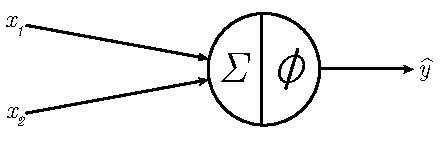
\includegraphics{images/neuron.pdf}
	\caption[Model of a McCulloch-Pitts-neuron]{Model of a McCulloch-Pitts-neuron. The inputs $x_i$ are summed up and put into the activation function $\phi$ whose result is the neuron's output $\hat{y}$.}
	\label{fig:neuron}
\end{figure}

Because numerical values are required for later operations, every logical value is transformed to 0 if it is false or 1 if it is true.
After summing up the inputs, a threshold activation function is applied.
In a mathematical sense
\begin{equation}
	\label{eq:neuron-mcculloch}
	\hat{y} = \phi \left( \sum_{i}^{n_x} x_i \right)
\end{equation}
describes this operation where $n_x$ is the number of inputs, $x_i$ a single input and $\phi$ the used activation function, in this case, the threshold activation function.
Plots of several activation functions including their equations are shown in \figref{fig:activation-functions}.
That means if a given threshold is reached the output of the perceptron is 1 and 0 otherwise.
This corresponds to the neurobiological spike of a neuron.
The truth tables for the logical AND and OR operations are shown in \tabref{tab:logical-operations}a and \tabref{tab:logical-operations}b, respectively.
The first one outputs true if all inputs are true.
The second one outputs true if at least one input is true.
It can be seen, that by changing the threshold value a different logical operation can be represented.
For two inputs a threshold of 2 represents the logical AND operation.
If the number of inputs is changed, a related change of the threshold still models the same operation.
In this example, the number of inputs is changed to 3 whereas the threshold must be changed to 3.
The same procedure is valid for the logical OR operation.
But here the threshold value is always 1 regardless of the number of inputs and therefore differs to other logical operations.
\begin{table}[]
	\centering
	\caption{Truth tables of logical operations}
	\label{tab:logical-operations}
	\begin{subtable}{.5\textwidth}
		\centering
		\caption{Logical AND}
		\label{tab:logical-and}
		\begin{tabular}{ccc|c|c}
			\hline
			$x_1$ & $x_2$ & $x_3$ & Thresh & Output \\ \hline
			0           & 0           &             & 2     & 0      \\
			0           & 1           &             & 2     & 0      \\
			1           & 0           &             & 2     & 0      \\
			1           & 1           &             & 2     & 1      \\ \hline
			0           & 1           & 1           & 3     & 0      \\
			1           & 1           & 1           & 3     & 1      \\
		\end{tabular}
	\end{subtable}%
	\begin{subtable}{.5\textwidth}
		\centering
		\caption{Logical OR}
		\label{tab:logical-or}
		\begin{tabular}{ccc|c|c}
			\hline
			$x_1$ & $x_2$ & $x_3$ & Thresh & Output \\ \hline
			0           & 0           &             & 1     & 0      \\
			0           & 1           &             & 1     & 1      \\
			1           & 0           &             & 1     & 1      \\
			1           & 1           &             & 1     & 1      \\ \hline
			0           & 0           & 0           & 1     & 0      \\
			0           & 0           & 1           & 1     & 1      \\
		\end{tabular}
	\end{subtable}
	
	\begin{subtable}{.5\textwidth}
		\centering
		\caption{Logical XOR}
		\label{tab:logical-xor}
		\begin{tabular}{ccc|c}
			\hline
			$x_1$ & $x_2$ & $x_3$ & Output 				\\ \hline
			0           & 0           &        & 0      \\
			0           & 1           &        & 1      \\
			1           & 0           &        & 1      \\
			1           & 1           &        & 0      \\ \hline
			0           & 1           & 1      & 0      \\
			1           & 1           & 1      & 1     
		\end{tabular}
	\end{subtable}%
	\begin{subtable}{.5\textwidth}
		\centering
		\caption{Logical XNOR}
		\label{tab:logical-xnor}
		\begin{tabular}{ccc|c}
			\hline
			$x_1$ & $x_2$ & $x_3$ & Output \\ \hline
			0           & 0           &             & 1      \\
			0           & 1           &             & 0      \\
			1           & 0           &             & 0      \\
			1           & 1           &             & 1      \\ \hline
			0           & 1           & 1           & 0      \\
			1           & 1           & 1           & 1     
		\end{tabular}
	\end{subtable}
\end{table}
One limitation of this neuron type is its inability to represent exclusive logical operations like XOR and XNOR \cite{Minsky69}, whose truth tables are shown in \tabref{tab:logical-operations}c and \tabref{tab:logical-operations}d, respectively.
The first one outputs true if the inputs are different.
The second one outputs true if all inputs are identical which equals an inverted XOR operation.
It can easily be seen, that no threshold value can be found for meeting the requirements.
For example, in the first case if the threshold is at 1 the first three combinations of inputs could be covered.
If all inputs are false the threshold value is not reached and therefore the neuron outputs a 0.
If the inputs differ from each other, the threshold value is reached which outputs a 1.
But as soon as the fourth one needs to be classified the threshold value is no longer valid.
The sum of the inputs equals two which exceeds the threshold and would output a logical true like in the OR case.
But according to the truth table, a logical false should be outputted.
The reasons for this misbehavior are the neuron's limitation to binary values and a threshold activation function and therefore the classification of only two categories.

Donald Hebb states "When an axon of cell A is near enough to excite a cell B and repeatedly or persistently takes part in firing it, some growth process or metabolic change takes place in one or both cells such that A's efficiency, as one of the cells firing B, is increased." \cite{Hebb1949} on how neurons learn.
This means, that if a neuron repeatedly and persistently stimulates a immediately subsequent neuron, i.e. the more often two wired neurons are active, their synaptic efficacy increases.
This is known as the Hebbian Theory.
Hebb summarizes this with his famous quote "neurons that fire together, wire together".

Frank Rosenblatt developed the first perceptron \cite{Rosenblatt58}.
Considering the Hebbian Theory the original McCulloch-Pitts-Neuron needs to be modified by adding associated weights for the inputs in order to simulate the strength of a synapse.
Thus, \eqref{eq:neuron-mcculloch} changes to
\begin{equation}
	\label{eq:neuron}
	\hat{y} = \phi \left( \sum_{i}^{n_x} x_i \cdot w_i \right)
\end{equation}
by considering the weights $w_i$.
Furthermore, the perceptron allows the usage of real-valued inputs and weights and uses the Heaviside step function as the activation function.
According to \figref{fig:heaviside-activation} the Heaviside function outputs 0 if its parameter is negative and 1 otherwise.
Therefore, its difference to the threshold activation function is just an offset of the threshold or bias, respectively.
Adapting \figref{fig:neuron} to this results in \figref{fig:perceptron}.
\begin{figure}
	\centering
	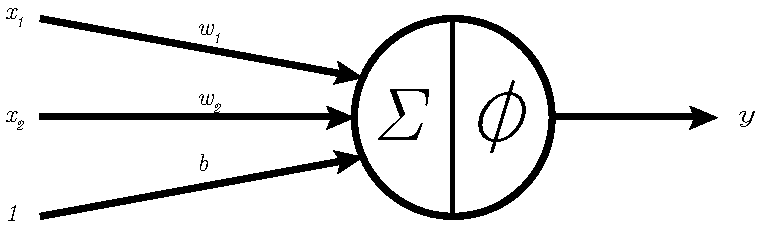
\includegraphics{images/perceptron}
	\caption[Model of a perceptron]{Model of a perceptron. The inputs $x_i$ are weighted by $w_i$ and are summed up with the bias $b$. This sum is put into the activation function $\phi$ whose result is the perceptron's output $\hat{y}$.}
	\label{fig:perceptron}
\end{figure}
There is one input with the value $1$ which is weighted by the bias.
Thus, when multiplied representing the bias.
This result is part of the weighted sum of the inputs which is fed to an activation function whose result is the output of the perceptron.
Combining this with \eqref{eq:neuron} yields
\begin{align}
	\label{eq:perceptron-sum}
	\hat{y} &= \phi \left( x_1 \cdot w_1 + x_2 \cdot w_2 + \ldots + x_{n_x} \cdot w_{n_x} + b \right)\\
	  &= \phi \left( \left( \sum_{i}^{n_x} x_i \cdot w_i \right) + b \right)
\end{align}
where $x_i$ are the inputs, $w_i$ the weights, $b$ the bias and $\phi$ the Heaviside activation function.
By changing the weights and biases, while keeping the inputs constant, a different behavior can be enforced.
In general, the inputs and weights are written as vectors of
\begin{align}
	\vec{x} &= \begin{pmatrix} x_1 & x_2 & \cdots & x_{n_x} \end{pmatrix}^T \\
	\vec{w} &= \begin{pmatrix} w_1 & w_2 & \cdots & w_{n_x} \end{pmatrix} 
\end{align}
for simplicity.
Inserting this in \eqref{eq:perceptron-sum} results in
\begin{equation}
	\label{eq:perceptron-activation}
	\hat{y} = \phi \left( \vec{w} \cdot \vec{x} + b \right)
\end{equation}
with the same parameters as before.
However, this model still works as a linear classifier and thus is unable to represent logical exclusive functions.
This can be solved by concatenating multiple perceptrons and building a multilayer artificial network.